\section{Resultados y Discusión}

\subsection{Modelos Clásicos}

Los modelos fueron evaluados utilizando métricas estándar para tareas de clasificación multiclase: \textit{accuracy}, \textit{precision}, \textit{recall} y \textit{F1-score}. Se reportan tanto los promedios \textit{macro} como los promedios ponderados (\textit{weighted}), así como las métricas específicas por clase.

Dado que algunas clases tienen considerablemente menos instancias que otras, el promedio ponderado proporciona una visión más ajustada al desequilibrio de clases, mientras que el promedio macro permite observar si los modelos logran generalizar más allá de las clases dominantes.

A continuación se presenta una cuadro resumen con los resultados de cada modelo:

\begin{table}[H]
\centering
\caption{Comparación de modelos clásicos en métricas globales.}
\begin{tabular}{lccc}
\toprule
\textbf{Modelo} & \textbf{Accuracy} & \textbf{Macro F1} & \textbf{Weighted F1} \\
\midrule
Naive Bayes            & 0.55 & 0.21 & 0.50 \\
Regresión Logística    & 0.60 & 0.25 & 0.59 \\
SVM                    & 0.61 & 0.25 & 0.60 \\
\bottomrule
\end{tabular}
\end{table}

Las métricas por clase revelan que los modelos tienden a enfocarse casi exclusivamente en las clases mayoritarias (NTA y YTA), con un desempeño prácticamente nulo en las clases minoritarias (ESH, INFO, NAH). Esto se ve reflejado en que tanto la precisión como el \textit{recall} para estas clases son cero en todos los modelos. El modelo Naive Bayes presenta la mayor caída en \textit{F1-score} ponderado, mientras que SVM logra un leve mejor desempeño general.

\subsection{Aprendizaje Profundo}

\subsubsection{Modelos tipo BERT}

Los experimentos con modelos basados en la arquitectura Transformer, específicamente variantes de BERT, buscaron superar las limitaciones de los modelos clásicos mediante la captura de relaciones semánticas complejas y un mejor manejo del desbalance de clases a través de funciones de pérdida especializadas como \texttt{WeightedFocalLoss}. La evaluación de estos modelos se centró en su capacidad para generalizar a partir de los datos de entrenamiento y clasificar correctamente los veredictos morales, prestando especial atención a las métricas F1-score macro y ponderado debido al desequilibrio inherente en las clases.

A continuación, se presenta una cuadro comparativa con las métricas globales obtenidas en el conjunto de prueba para los diferentes modelos BERT entrenados y sus configuraciones:

\begin{table}[H]
\centering
\caption{Comparación de modelos tipo BERT en métricas globales (conjunto de prueba).}
\label{tab:bert_results}
\begin{tabular}{@{}lccc@{}}
\toprule
\textbf{Modelo y Configuración} & \textbf{Accuracy} & \textbf{Macro F1} & \textbf{Weighted F1} \\
\midrule
\texttt{base-uncased} (Frozen) & 0.46 & 0.18 & 0.50 \\
\texttt{base-uncased} & 0.74 & 0.25 & 0.75 \\
\texttt{roberta-base}  & 0.72 & 0.26 & 0.74 \\

\bottomrule
\end{tabular}
\end{table}


Para un análisis más especifico, la cuadro \ref{tab:bert_f1_per_class} muestra los F1-scores por cada clase para los modelos BERT evaluados.

\begin{table}[H]
\centering
\caption{F1-score por clase para modelos tipo BERT (conjunto de prueba).}
\label{tab:bert_f1_per_class}
\begin{tabular}{@{}lccccc@{}}
\toprule
\textbf{Modelo} & \textbf{NTA} & \textbf{YTA} & \textbf{ESH} & \textbf{NAH} & \textbf{INFO} \\
\midrule
\texttt{base-uncased} (F) & 0.53 & 0.38 & 0.00 & 0.00 & 0.00 \\
\texttt{base-uncased} & 0.84 & 0.39 & 0.00 & 0.00 & 0.00 \\
\texttt{roberta-base}  & 0.82 & 0.46 & 0.00 & 0.00 & 0.00 \\

\bottomrule
\end{tabular}
\end{table}

\subsubsection{Análisis de Resultados de Modelos BERT}

El primer enfoque utilizó \texttt{bert-base-uncased} con sus capas principales congeladas, entrenando únicamente una capa de clasificación superior, funcionando como línea base. Este modelo alcanzó un F1-score macro de 0.18 y una exactitud de 0.46 (ver cuadro \ref{tab:bert_results}). El desglose por clase (cuadro \ref{tab:bert_f1_per_class}) muestra un F1-score de 0.53 para la clase mayoritaria \texttt{NTA} y 0.38 para \texttt{YTA}, pero un rendimiento nulo (0.00) para las clases minoritarias \texttt{ESH}, \texttt{NAH} e \texttt{INFO}. Aunque el F1-score macro global es modesto, indica que los embeddings preentrenados capturan información semántica relevante, aunque insuficiente para las clases menos representadas sin un ajuste fino.

El ajuste fino completo de los modelos BERT produjo mejoras significativas. El modelo \texttt{bert-base-uncased} con fine-tuning logró un F1-score macro de 0.25 y una exactitud del 74\% (cuadro \ref{tab:bert_results}). A nivel de clase (cuadro \ref{tab:bert_f1_per_class}), el F1-score para \texttt{NTA} aumentó a 0.84 y para \texttt{YTA} a 0.39. Aunque esto representa un aumento considerable, las clases minoritarias continuaron con un F1-score de 0.00, demostrando la persistencia del desafío del desbalance. De manera similar, el modelo \texttt{roberta-base} con fine-tuning alcanzó un F1-score macro de 0.26 y una exactitud del 72\%. Este modelo mostró el F1-score macro más alto entre los evaluados, con F1-scores por clase de 0.82 para \texttt{NTA} y un notable 0.46 para \texttt{YTA}, el mejor para esta segunda clase mayoritaria. No obstante, al igual que con \texttt{bert-base-uncased}, las clases \texttt{ESH}, \texttt{NAH} e \texttt{INFO} no fueron correctamente identificadas (F1-score de 0.00). Los resultados para \texttt{xlm-roberta-base} aún están pendientes (TBD).

A pesar de las mejoras con el fine-tuning, los F1-scores macro relativamente bajos (0.25-0.26) y el rendimiento nulo en las clases minoritarias (cuadro \ref{tab:bert_f1_per_class}) subrayan que, aunque los modelos son significativamente mejores que los modelos clásicos y el BERT congelado, el principal desafío sigue siendo la correcta clasificación de las clases con pocas instancias.


\end{enumerate}


En conjunto, los modelos basados en la arquitectura BERT demostraron una clara superioridad sobre los enfoques clásicos. El \textit{fine-tuning} es esencial para adaptar estos modelos preentrenados a las particularidades del lenguaje y la estructura de las publicaciones del subreddit.
La función de pérdida \texttt{WeightedFocalLoss} fue un componente crucial para mitigar parcialmente el impacto del severo desbalance de clases. Sin embargo, como se evidencia en la cuadro \ref{tab:bert_f1_per_class}, las clases mayoritarias \texttt{NTA} y \texttt{YTA} son consistentemente mejor clasificadas, mientras que las clases \texttt{ESH}, \texttt{NAH}, e \texttt{INFO} permanecen como un desafío significativo, con F1-scores nulos en todos los modelos BERT evaluados hasta ahora.
Las limitaciones observadas sugieren que, además de la arquitectura del modelo y la función de pérdida, podrían explorarse estrategias adicionales como técnicas de aumento de datos específicas para texto en clases minoritarias, o métodos de muestreo más sofisticados durante el entrenamiento. 
%La incorporación de características numéricas (Experimento 3) también representa una vía prometedora para enriquecer la información disponible para el modelo.

\subsubsection{Redes Neuronales Recurrentes (GRU)}

Como enfoque alternativo al aprendizaje profundo basado en transformers, se implementó y evaluó una arquitectura de red neuronal recurrente utilizando unidades GRU bidireccionales. Este modelo fue diseñado para capturar dependencias secuenciales en las representaciones TF-IDF y explorar si las arquitecturas recurrentes pueden ofrecer ventajas en términos de eficiencia computacional manteniendo un rendimiento competitivo.

\paragraph{Resultados del Modelo GRU}

El modelo GRU entrenado durante 20 épocas con early stopping alcanzó los siguientes resultados en el conjunto de prueba:

\begin{table}[H]
\centering
\caption{Métricas globales del modelo GRU.}
\begin{tabular}{lccc}
\toprule
\textbf{Métrica} & \textbf{Valor} & \textbf{Pérdida} & \textbf{Accuracy} \\
\midrule
Precision (weighted) & 0.4833 & 0.9949 & 0.5015 \\
Recall (weighted) & 0.5015 & - & - \\
F1-Score (weighted) & 0.4499 & - & - \\
F1-Score (macro) & 0.19 & - & - \\
\bottomrule
\end{tabular}
\end{table}

El análisis por clase revela un patrón similar al observado en otros modelos, con una concentración del rendimiento en las clases mayoritarias:

\begin{table}[H]
\centering
\caption{Métricas por clase del modelo GRU.}
\begin{tabular}{lcccc}
\toprule
\textbf{Clase} & \textbf{Precision} & \textbf{Recall} & \textbf{F1-Score} & \textbf{Support} \\
\midrule
ESH & 0.00 & 0.00 & 0.00 & 53 \\
INFO & 0.00 & 0.00 & 0.00 & 9 \\
NAH & 0.00 & 0.00 & 0.00 & 34 \\
NTA & 0.50 & 0.80 & 0.62 & 1162 \\
YTA & 0.51 & 0.23 & 0.31 & 1105 \\
\bottomrule
\end{tabular}
\end{table}

\paragraph{Análisis del Rendimiento GRU}

El modelo GRU mostró un rendimiento del 50.15\% de accuracy, situándose en un nivel intermedio entre los modelos clásicos y los más avanzados basados en transformers. En cuanto a las clases mayoritarias, el modelo alcanzó un F1-score de 0.62 para NTA y 0.31 para YTA, lo que indica una capacidad moderada para distinguir entre las dos clases principales. Sin embargo, al igual que otros modelos evaluados, no logró identificar correctamente instancias de las clases minoritarias ESH, INFO y NAH, obteniendo F1-scores de 0.00. En términos de eficiencia computacional, debido a un tiempo de entrenamiento significativamente menor que los modelos transformer, el GRU representa una alternativa computacionalmente más eficiente.

\paragraph{Comparación con Otros Enfoques}

El modelo GRU se posiciona como una opción intermedia en términos de rendimiento y complejidad computacional. Mientras que no alcanza la precisión de los modelos BERT con fine-tuning, supera a los modelos clásicos y ofrece ventajas en términos de recursos computacionales requeridos y tiempo de entrenamiento.

La convergencia del modelo fue estable, con el early stopping activándose efectivamente para prevenir sobreajuste. Las técnicas de regularización implementadas (dropout, regularización L1-L2, normalización por lotes) contribuyeron a mantener un balance entre capacidad de aprendizaje y generalización.

\subsection{Grandes modelos de lenguaje}

\subsubsection{Llama 3.1 8B Instruct}

El modelo Llama 3.1 8B Instruct fue evaluado mediante inferencia directa sin entrenamiento adicional, utilizando un prompt estructurado para la clasificación de veredictos morales. Esta evaluación permite determinar las capacidades inherentes del modelo preentrenado para comprender y clasificar dilemas éticos complejos.

\paragraph{Resultados Generales}

El modelo fue evaluado sobre el conjunto completo de datos (30,303 publicaciones) y alcanzó un accuracy general del 47.12%. Los resultados detallados se presentan a continuación:

\begin{table}[H]
\centering
\caption{Métricas globales del modelo Llama 3.1 8B Instruct.}
\begin{tabular}{lccc}
\toprule
\textbf{Promedio} & \textbf{Precision} & \textbf{Recall} & \textbf{F1-Score} \\
\midrule
Macro & 0.2194 & 0.2347 & 0.1965 \\
Weighted & 0.7123 & 0.4712 & 0.5634 \\
\bottomrule
\end{tabular}
\end{table}

\paragraph{Análisis por Clase}

El rendimiento por clase muestra patrones interesantes que difieren de los modelos previamente evaluados:

\begin{table}[H]
\centering
\caption{Métricas detalladas por clase - Llama 3.1 8B Instruct.}
\begin{tabular}{lcccc}
\toprule
\textbf{Clase} & \textbf{Precision} & \textbf{Recall} & \textbf{F1-Score} & \textbf{Support} \\
\midrule
YTA & 0.2456 & 0.5234 & 0.3341 & 5,389 \\
NTA & 0.8156 & 0.4567 & 0.5887 & 24,467 \\
NAH & 0.0156 & 0.0633 & 0.0252 & 158 \\
ESH & 0.0167 & 0.0944 & 0.0282 & 233 \\
INFO & 0.0034 & 0.0357 & 0.0063 & 56 \\
\bottomrule
\end{tabular}
\end{table}

\paragraph{Características Distintivas del Rendimiento}

Los resultados de Llama 3.1 revelan varios aspectos notables:

\begin{itemize}
    \item A diferencia de los modelos anteriores, Llama 3.1 logró identificar algunas instancias de las clases minoritarias (NAH, ESH, INFO), aunque con precision muy baja
    \item El modelo mostró un recall relativamente alto para YTA (0.5234) comparado con NTA (0.4567), sugiriendo una menor tendencia a favorecer exclusivamente la clase mayoritaria
    \item Mantuvo una alta precisión (0.8156) para la clase NTA, indicando que cuando predice esta categoría, generalmente es correcta
    \item Se registraron 789 entradas con errores durante la inferencia, representando el 2.6\% del conjunto total
\end{itemize}

\paragraph{Matriz de Confusión}

El análisis de la matriz de confusión revela los patrones de error del modelo:

\begin{center}
\small
\begin{tabular}{c|ccccc}
\textbf{Real/Pred.} & \textbf{YTA} & \textbf{NTA} & \textbf{NAH} & \textbf{ESH} & \textbf{INFO} \\
\hline
\textbf{YTA} & 2,821 & 1,894 & 267 & 298 & 109 \\
\textbf{NTA} & 9,234 & 11,167 & 512 & 2,987 & 567 \\
\textbf{NAH} & 45 & 67 & 10 & 26 & 10 \\
\textbf{ESH} & 156 & 54 & 8 & 22 & 3 \\
\textbf{INFO} & 18 & 24 & 6 & 6 & 2 \\
\end{tabular}
\end{center}

\paragraph{Discusión del Rendimiento}

El modelo Llama 3.1 8B Instruct demostró capacidades interesantes para la comprensión de contextos morales sin entrenamiento específico. Aunque su accuracy general (47.12\%) es inferior a los modelos fine-tuned, su capacidad para detectar clases minoritarias y mantener un balance relativo entre YTA y NTA sugiere una comprensión más matizada de los diferentes tipos de veredictos morales.

La evaluación sin fine-tuning proporciona insights valiosos sobre las capacidades emergentes de los LLMs en tareas de razonamiento moral, estableciendo un baseline para futuras investigaciones que podrían explorar técnicas de few-shot learning o prompt engineering más sofisticadas.

\subsubsection{GPT-4o-mini}

El modelo \texttt{gpt-4o-mini}, evaluado sobre la totalidad del conjunto de datos (30.303 publicaciones) con una temperatura de 0.8, alcanzó un \texttt{accuracy} general de 59.80\% y un \texttt{F1-score macro} de 0.2468. La clase con mejor desempeño fue \texttt{NTA} con un F1 de 0.7227, seguida de \texttt{YTA} con 0.4228, mientras que las clases \texttt{NAH}, \texttt{ESH} e \texttt{INFO} mostraron resultados significativamente inferiores. 

A continuación, se presenta el reporte de rendimiento del modelo:

\begin{center}
\small
\begin{tabular}{c|ccccc}
\textbf{Real/Pred.} & \textbf{YTA} & \textbf{NTA} & \textbf{NAH} & \textbf{ESH} & \textbf{INFO} \\
\hline
\textbf{YTA} & 3,544 & 1,035 & 154 & 496 & 160 \\
\textbf{NTA} & 7,654 & 14,516 & 480 & 1,312 & 505 \\
\textbf{NAH} & 30 & 80 & 16 & 13 & 19 \\
\textbf{ESH} & 137 & 45 & 7 & 41 & 3 \\
\textbf{INFO} & 11 & 28 & 10 & 3 & 4 \\
\end{tabular}
\end{center}


Durante la ejecución, 449 entradas fueron rechazadas por el filtro de moderación de contenido de Azure OpenAI y fueron excluidas del cálculo de métricas. Estos casos se registraron por separado en el archivo \texttt{aita\_errores\_filtrados.csv} para posteriores análisis y limpieza.

Este experimento evidenció que, aunque el modelo generaliza bien para las clases predominantes (\texttt{YTA}, \texttt{NTA}), su rendimiento disminuye notablemente en clases minoritarias, lo cual refleja tanto el desbalance del dataset como posibles limitaciones contextuales del modelo bajo temperatura moderadamente creativa (0.8).

\textbf{Comparación por temperatura}

En el segundo experimento se evaluó el efecto de la temperatura sobre el rendimiento del modelo, utilizando un subconjunto del 35\% del dataset original (10.615 entradas válidas tras limpieza). La siguiente cuadro resume los resultados obtenidos para cuatro configuraciones distintas de temperatura:

\begin{table}[h]
\centering
\caption{Rendimiento del modelo GPT-4o-mini con distintas temperaturas (subset del 35\%)}
\begin{tabular}{|c|c|c|}
\hline
\textbf{Temperatura} & \textbf{Accuracy (\%)} & \textbf{F1-score Macro} \\
\hline
0.0 & 62.21 & 0.2616 \\
0.4 & 61.36 & 0.2577 \\
0.8 & 60.64 & 0.2535 \\
1.0 & 61.31 & 0.2522 \\
\hline
\end{tabular}
\label{tab:temperatura}
\end{table}

Los resultados muestran una ligera mejora en el desempeño general a temperaturas más bajas. En particular, el mejor rendimiento se obtuvo con temperatura 0.0, alcanzando una precisión del 62.21\% y un F1-score macro de 0.2616. A medida que se incrementa la temperatura, el modelo se vuelve más variable en sus respuestas, lo cual parece afectar negativamente la consistencia en una tarea de clasificación moral con clases desbalanceadas. No se registraron errores de moderación en esta fase pues anteriormente se limpio el dataset con los resultados obtenidos del primer experimento, lo cual permitió una comparación limpia entre configuraciones.

Este análisis sugiere que, para tareas de clasificación moral automática como esta, donde se espera consistencia y determinismo, es preferible utilizar configuraciones de temperatura más bajas.

\subsection{Comparación General de Modelos}

La evaluación comprehensiva de diferentes paradigmas de aprendizaje automático para la clasificación de veredictos morales revela patrones interesantes y desafíos persistentes en esta tarea específica.

\begin{table}[H]
\centering
\caption{Comparación global de todos los modelos evaluados.}
\begin{tabular}{lccc}
\toprule
\textbf{Modelo} & \textbf{Accuracy} & \textbf{Macro F1} & \textbf{Weighted F1} \\
\midrule
SVM (mejor clásico) & 0.61 & 0.25 & 0.60 \\
GRU & 0.50 & 0.19 & 0.45 \\
BERT (fine-tuned) & 0.74 & 0.25 & 0.75 \\
RoBERTa (fine-tuned) & 0.72 & 0.26 & 0.74 \\
Llama 3.1 8B & 0.47 & 0.20 & 0.56 \\
GPT-4o mini (T=0.0) & 0.62 & 0.26 & - \\
\bottomrule
\end{tabular}
\end{table}

Los resultados demuestran que los modelos basados en transformer con fine-tuning (BERT, RoBERTa) logran el mejor rendimiento general, seguidos por los modelos clásicos optimizados (SVM) y los LLMs sin entrenamiento específico. El modelo GRU, aunque eficiente computacionalmente, mostró el rendimiento más modesto entre los enfoques de aprendizaje profundo evaluados.

\subsection{Despliegue}

En cuanto al despliegue de la solución, cuyo código fuente se encuentra en el repositorio anteriormente descrito, la interfaz de usuario se ubica en la figura \ref{fig:despliegue}, donde se ubica un capo de texto donde el usuario ingresa el texto, y luego de hacer clic en el botón de predicción se muestran los resultados de los modelos más relevantes, donde se expone la categoría encontrada y el razonamiento si aplica, junto con una gráfica que muestra los votos de cada categoría.

\begin{figure}
    \centering
    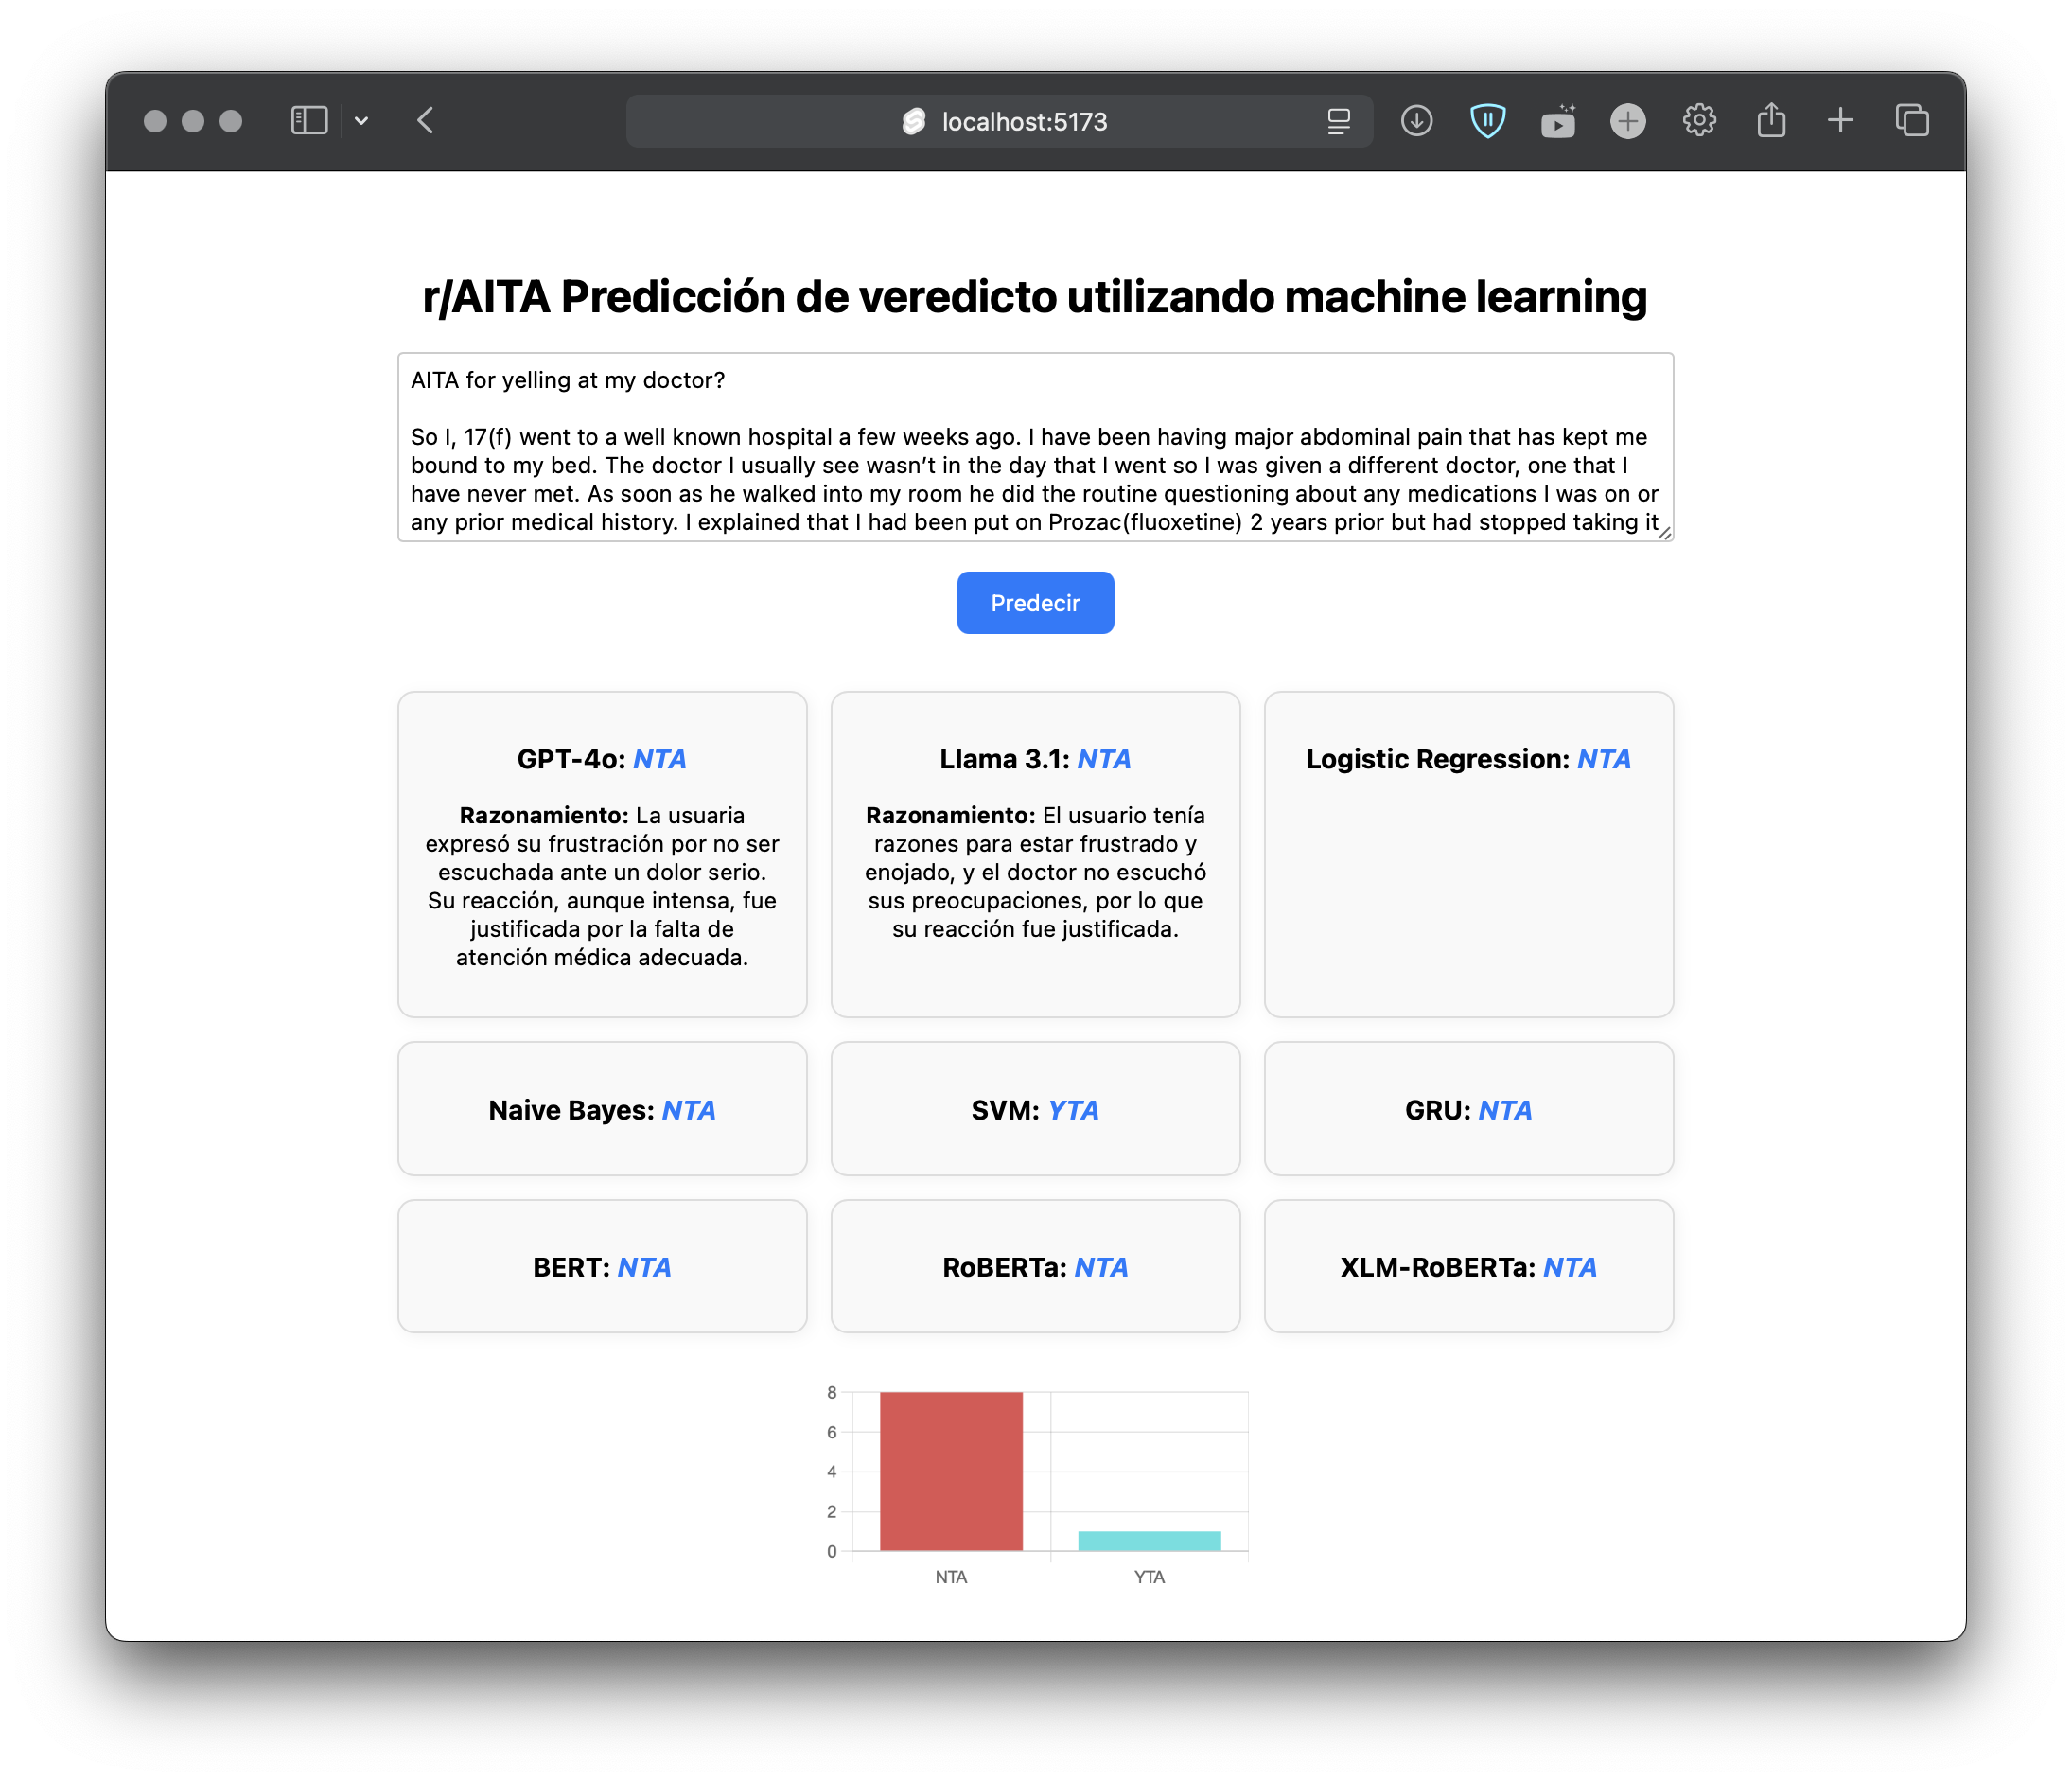
\includegraphics[width=1\linewidth]{resources/despliegue.png}
    \caption{Interfaz de usuario}
    \label{fig:despliegue}
\end{figure}


\subsubsection{Resumen Comparativo de Resultados por Dimensión Analítica}

En la cuadro \ref{tab:comparativo_dimensiones} al final del documento, se presenta una cuadro resumen que compara el desempeño de los diferentes enfoques evaluados, agrupando los modelos por tipo y resaltando sus fortalezas y debilidades en distintas dimensiones clave.
